\subsection{Validazione e Collaudo}
\label{validazione_e_collaudo}
\textbf{Periodo:} dal 2020-04-10 al 2020-05-09

La fase inizia appena conclusa la precedente e termina con la \textit{Revisione di Accettazione.}

Le precondizioni sono:
\begin{itemize}
    \item Le postcondizioni della fase precedente sono state soddisfatte;
\end{itemize}

Le postcondizioni sono:
\begin{itemize}
    \item Aggiornamento e correzione documenti già prodotti;
    \item Esecuzione dei vari test;
    \item Completamento del prodotto in base a quanto discusso in \textit{Revisione di Qualifica};
    \item Consegna dei documenti richiesti in entrata alla \textit{Revisione di Accettazione};
    \item Ultimata preparazione della presentazione da esporre in sede di revisione.
\end{itemize}

E' composta da nove incrementi e una nuova attività:
\begin{itemize}
    \item \textbf{Incremento e Verifica}: alcuni dei documenti già prodotti vengono migliorati e aggiornati (\textit{\NdP}, \textit{\PdP}, \textit{Glossario},\textit{\PdQ}, \textit{\AdR}, \textit{Technology Baseline}, \textit{Product Baseline}, \textit{Specifica Tecnica}, \textit{Codifica}, \textit{Manuale Utente}); 
    \item \textbf{Validazione e Collaudo}: Realizzazione degli ultimi test, con successivi controlli finali per garantire un buon livello di qualità e correttezza
\end{itemize}

\newpage
\subsubsection{Diagramma di Gantt: Validazione e Collaudo}
\begin{figure}[ht]
    \centering
    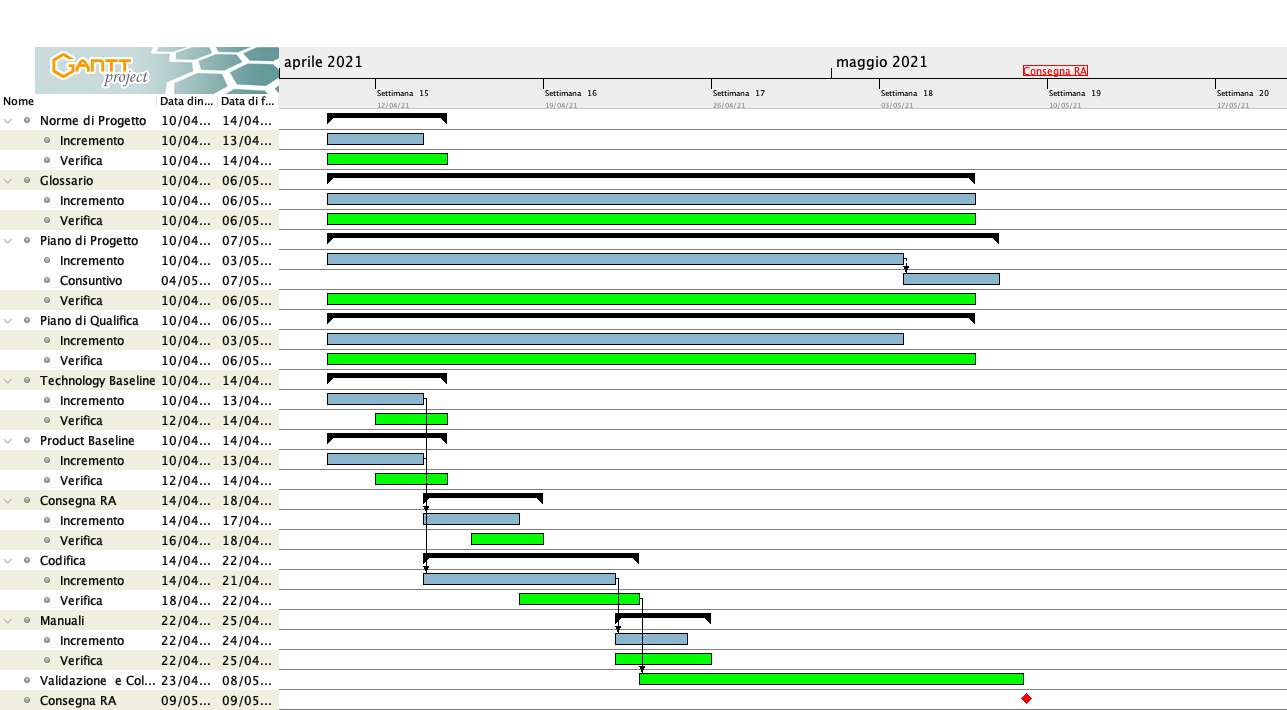
\includegraphics[width=\textwidth]{../../Immagini/GanttValidazioneECollaudo}
    \caption{Diagramma di Gantt dell'avvitià di Validazione e Collaudo}
\end{figure}